%-------------------------------------------
% En-tête type de document pour le projet PLD
% Il suffit de remplir le input ligne 45
%-------------------------------------------

\documentclass[a4paper]{article}

\usepackage[utf8]{inputenc}   
\usepackage[top=2cm, bottom=2cm, left=2cm, right=2cm]{geometry}
\usepackage{ucs}
% Reconnaitre les caratères accentués dans le source.
\usepackage[T1]{fontenc} 
\usepackage{lmodern}
\usepackage[francais]{babel}
% Insertion d'images
\usepackage{graphicx}
% Utilisation du symbole EURO
\usepackage{eurosym}

\setlength{\parskip}{10pt plus 1pt minus 1pt}

\begin{document}

%------------------------------------- Page de titre
\begin{titlepage}
~ 
\vfill
	\begin{center}
		\begin{Huge}
		Projet D'ingénierie : Procédure de découpage d'un système en sous-systèmes\\
		\end{Huge} 
\vfill
		\textbf{Hexanome 4111 :} 
		\\Quentin \bsc{Calvez}, Matthieu \bsc{Coquet}, 
		\\Jan \bsc{Keromnes}, Alexandre \bsc{Lefoulon}, 
		\\Thaddée \bsc{Tyl}, Xavier \bsc{Sauvagnat},
		\\Tuuli \bsc{Tyrväinen}
\vfill		
		\begin{Large}
		Janvier 2012
		\end{Large}
\vfill
	\begin{tabular}{|c|c|c|c|c|}
 	 \hline
   Destinataire & Version & Etat & Dernière révision & Equipe \\
   \hline
   Client & 1 & Validé & \today & H4111 \\
   \hline
	\end{tabular}
	\end{center}
\vfill
\end{titlepage}
%----------------------------------------------------
%--------------------------------- Table des matières
\newpage
\tableofcontents
\newpage
%----------------------------------------------------

%------------------- Insertion du contenu du document
\section{Presentation}
\subsection{Objet}
Ce document détaille les étapes nécessaires à la décomposition d'un système complexe en sous-systèmes. Ce découpage permettant ainsi de dégager des sous projets pouvant être de natures différentes au sein du système complet. Dans une analyse exhaustive du sytème, il serait nécéssaire d'établir un cahier des charges pour chaque sous projet identifié.
\medskip

\subsection{Domaine d'application}
Ce document, rédigé par le chef de projet doit être une aide au Groupe d'Etudes Informatiques chargé de décomposer (en collaboration avec le chef de projet) le système à concevoir afin d'en dégager des sous-projets et enfin des cahiers des charges à rédiger pour chaque sous-projet.
\subsection{Description}
Avant tout découpage, il s'agit d'avoir une vision précise et critique du projet. Le GEI doit de même toujours avoir en tête les besoins fonctionnels et non fonctionnels du client. L'élaboration précédente de l'architecture  ainsi que de la conception générale du système permet d'avoir appréhendé les difficultés liées au système. 
\medskip
Comment avons nous procédé de manière pratique ?
\medskip
Il est important pour ce type d'exercice, d'avoir l'avis de l'ensemble du GEI car chaque ressource emmet son propre point de vue, sa propre \og projection \fg du système. Le groupe composé du GEI et du chef de projet peut donc se réunir autour d'un tableau noir. Sous l'oeil du RQ, le chef de projet doit être l'animateur de la séance de découpage, il peut donc être celui qui se charge d'écrire au tableau. Tout en écrivant les découpages suggérés par ces collègue il tempère et mène le brainstorming. Il doit pour chaque idée délivrée repeser les pour et les contres et les discuter avec le reste du groupe. L'utilisation de couleurs différentes pour les systèmes, sous-systèmes et sous-projets est primordiale, elle permet au GEI de bien cerner les différents niveaux de granularité. Le CdP peut ensuite laisser le GEI se répartir les cahiers des charges ainsi définit en fonction des affinités et des compétences de chacun.
\subsection{Références}
Ce document aide à la rédaction du :
\begin{itemize}
\item Plan de management de projet
\item Cahier des charges
\end{itemize}

\medskip 

La rédaction de ce document a été aidée par :
\begin{itemize}
\item Cours de Regis Aubry
\item Best Practice : Rédaction d'une procédure par le RQ
\end{itemize}


\section{Logigramme et notions utiles}
\subsection{Logigramme}
\begin {center}
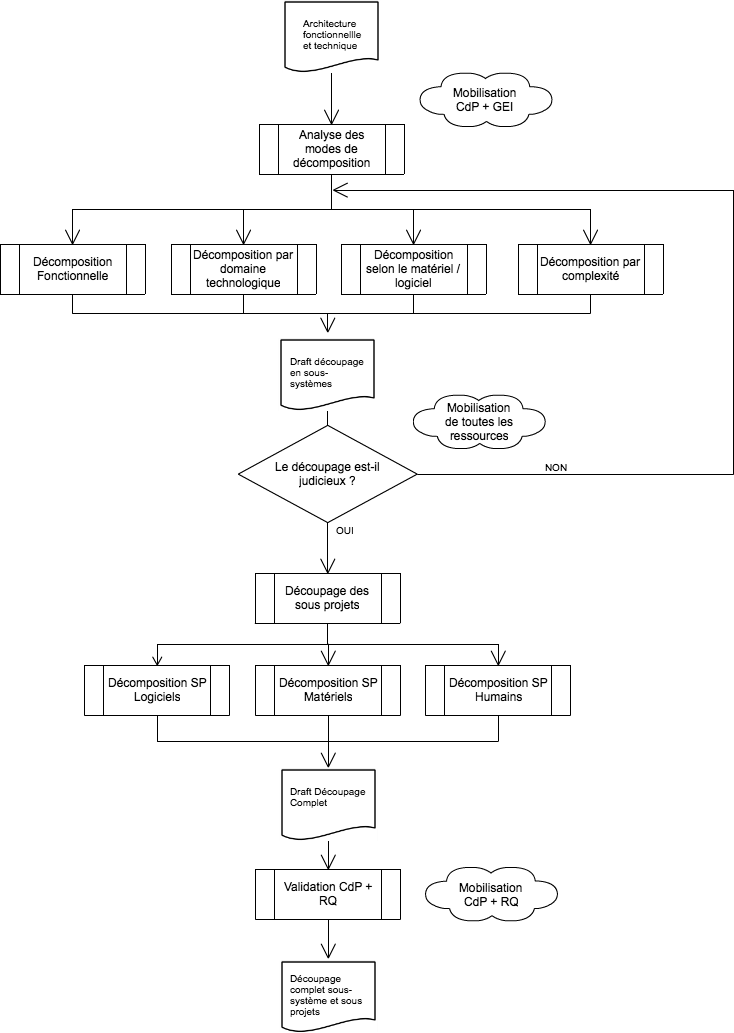
\includegraphics[width=\textwidth]{png/DecompositionSousSystem.png}
\end {center}

\subsection{Principes de découpe en sous-projets}
En ce qui concerne la décomposition en sous-projets, il est possible de considérer plusieurs approches :
\begin{itemize}
\item Un sous-système va donner lieu à un sous projet : rarement utilisé dans notre cas d'étude car nos sous-systèmes sont assez généraux.
\item Un sous-système va donner lieu à plusieurs sous-projets : souvent utilisé dans notre cas d'étude, pour chaque sous-système, nous définissons plusieurs sous-projet qui donneront donc lieu à plusieurs cahiers des charges.
\item Plusieurs sous-systèmes vont se réunir pour générer un ou plusieurs sous-projets : Il est parfois intéressant, pour des notions qui ne sont pas présentes explicitement en tant que sous-systèmes de pouvoir les représenter en les faisant apparaître dans des sous-projet.
\end{itemize}



%----------------------------------------------------

\end{document}
